% Options for packages loaded elsewhere
\PassOptionsToPackage{unicode}{hyperref}
\PassOptionsToPackage{hyphens}{url}
%
\documentclass[
]{book}
\usepackage{amsmath,amssymb}
\usepackage{lmodern}
\usepackage{iftex}
\ifPDFTeX
  \usepackage[T1]{fontenc}
  \usepackage[utf8]{inputenc}
  \usepackage{textcomp} % provide euro and other symbols
\else % if luatex or xetex
  \usepackage{unicode-math}
  \defaultfontfeatures{Scale=MatchLowercase}
  \defaultfontfeatures[\rmfamily]{Ligatures=TeX,Scale=1}
\fi
% Use upquote if available, for straight quotes in verbatim environments
\IfFileExists{upquote.sty}{\usepackage{upquote}}{}
\IfFileExists{microtype.sty}{% use microtype if available
  \usepackage[]{microtype}
  \UseMicrotypeSet[protrusion]{basicmath} % disable protrusion for tt fonts
}{}
\makeatletter
\@ifundefined{KOMAClassName}{% if non-KOMA class
  \IfFileExists{parskip.sty}{%
    \usepackage{parskip}
  }{% else
    \setlength{\parindent}{0pt}
    \setlength{\parskip}{6pt plus 2pt minus 1pt}}
}{% if KOMA class
  \KOMAoptions{parskip=half}}
\makeatother
\usepackage{xcolor}
\usepackage{color}
\usepackage{fancyvrb}
\newcommand{\VerbBar}{|}
\newcommand{\VERB}{\Verb[commandchars=\\\{\}]}
\DefineVerbatimEnvironment{Highlighting}{Verbatim}{commandchars=\\\{\}}
% Add ',fontsize=\small' for more characters per line
\usepackage{framed}
\definecolor{shadecolor}{RGB}{248,248,248}
\newenvironment{Shaded}{\begin{snugshade}}{\end{snugshade}}
\newcommand{\AlertTok}[1]{\textcolor[rgb]{0.94,0.16,0.16}{#1}}
\newcommand{\AnnotationTok}[1]{\textcolor[rgb]{0.56,0.35,0.01}{\textbf{\textit{#1}}}}
\newcommand{\AttributeTok}[1]{\textcolor[rgb]{0.77,0.63,0.00}{#1}}
\newcommand{\BaseNTok}[1]{\textcolor[rgb]{0.00,0.00,0.81}{#1}}
\newcommand{\BuiltInTok}[1]{#1}
\newcommand{\CharTok}[1]{\textcolor[rgb]{0.31,0.60,0.02}{#1}}
\newcommand{\CommentTok}[1]{\textcolor[rgb]{0.56,0.35,0.01}{\textit{#1}}}
\newcommand{\CommentVarTok}[1]{\textcolor[rgb]{0.56,0.35,0.01}{\textbf{\textit{#1}}}}
\newcommand{\ConstantTok}[1]{\textcolor[rgb]{0.00,0.00,0.00}{#1}}
\newcommand{\ControlFlowTok}[1]{\textcolor[rgb]{0.13,0.29,0.53}{\textbf{#1}}}
\newcommand{\DataTypeTok}[1]{\textcolor[rgb]{0.13,0.29,0.53}{#1}}
\newcommand{\DecValTok}[1]{\textcolor[rgb]{0.00,0.00,0.81}{#1}}
\newcommand{\DocumentationTok}[1]{\textcolor[rgb]{0.56,0.35,0.01}{\textbf{\textit{#1}}}}
\newcommand{\ErrorTok}[1]{\textcolor[rgb]{0.64,0.00,0.00}{\textbf{#1}}}
\newcommand{\ExtensionTok}[1]{#1}
\newcommand{\FloatTok}[1]{\textcolor[rgb]{0.00,0.00,0.81}{#1}}
\newcommand{\FunctionTok}[1]{\textcolor[rgb]{0.00,0.00,0.00}{#1}}
\newcommand{\ImportTok}[1]{#1}
\newcommand{\InformationTok}[1]{\textcolor[rgb]{0.56,0.35,0.01}{\textbf{\textit{#1}}}}
\newcommand{\KeywordTok}[1]{\textcolor[rgb]{0.13,0.29,0.53}{\textbf{#1}}}
\newcommand{\NormalTok}[1]{#1}
\newcommand{\OperatorTok}[1]{\textcolor[rgb]{0.81,0.36,0.00}{\textbf{#1}}}
\newcommand{\OtherTok}[1]{\textcolor[rgb]{0.56,0.35,0.01}{#1}}
\newcommand{\PreprocessorTok}[1]{\textcolor[rgb]{0.56,0.35,0.01}{\textit{#1}}}
\newcommand{\RegionMarkerTok}[1]{#1}
\newcommand{\SpecialCharTok}[1]{\textcolor[rgb]{0.00,0.00,0.00}{#1}}
\newcommand{\SpecialStringTok}[1]{\textcolor[rgb]{0.31,0.60,0.02}{#1}}
\newcommand{\StringTok}[1]{\textcolor[rgb]{0.31,0.60,0.02}{#1}}
\newcommand{\VariableTok}[1]{\textcolor[rgb]{0.00,0.00,0.00}{#1}}
\newcommand{\VerbatimStringTok}[1]{\textcolor[rgb]{0.31,0.60,0.02}{#1}}
\newcommand{\WarningTok}[1]{\textcolor[rgb]{0.56,0.35,0.01}{\textbf{\textit{#1}}}}
\usepackage{longtable,booktabs,array}
\usepackage{calc} % for calculating minipage widths
% Correct order of tables after \paragraph or \subparagraph
\usepackage{etoolbox}
\makeatletter
\patchcmd\longtable{\par}{\if@noskipsec\mbox{}\fi\par}{}{}
\makeatother
% Allow footnotes in longtable head/foot
\IfFileExists{footnotehyper.sty}{\usepackage{footnotehyper}}{\usepackage{footnote}}
\makesavenoteenv{longtable}
\usepackage{graphicx}
\makeatletter
\def\maxwidth{\ifdim\Gin@nat@width>\linewidth\linewidth\else\Gin@nat@width\fi}
\def\maxheight{\ifdim\Gin@nat@height>\textheight\textheight\else\Gin@nat@height\fi}
\makeatother
% Scale images if necessary, so that they will not overflow the page
% margins by default, and it is still possible to overwrite the defaults
% using explicit options in \includegraphics[width, height, ...]{}
\setkeys{Gin}{width=\maxwidth,height=\maxheight,keepaspectratio}
% Set default figure placement to htbp
\makeatletter
\def\fps@figure{htbp}
\makeatother
\setlength{\emergencystretch}{3em} % prevent overfull lines
\providecommand{\tightlist}{%
  \setlength{\itemsep}{0pt}\setlength{\parskip}{0pt}}
\setcounter{secnumdepth}{5}
\usepackage{booktabs}
\ifLuaTeX
  \usepackage{selnolig}  % disable illegal ligatures
\fi
\usepackage[]{natbib}
\bibliographystyle{plainnat}
\IfFileExists{bookmark.sty}{\usepackage{bookmark}}{\usepackage{hyperref}}
\IfFileExists{xurl.sty}{\usepackage{xurl}}{} % add URL line breaks if available
\urlstyle{same} % disable monospaced font for URLs
\hypersetup{
  pdftitle={Metacell Tutorial},
  pdfauthor={Mariia Bilous, Léonard Hérault, Aurélie Gabriel, David Gfeller},
  hidelinks,
  pdfcreator={LaTeX via pandoc}}

\title{Metacell Tutorial}
\author{Mariia Bilous, Léonard Hérault, Aurélie Gabriel, David Gfeller}
\date{2023-07-28}

\begin{document}
\maketitle

{
\setcounter{tocdepth}{1}
\tableofcontents
}
\hypertarget{about}{%
\chapter{About}\label{about}}

The structure of this tutorial.

\hypertarget{book-structure}{%
\section{Book structure}\label{book-structure}}

Book consists of several Chapters (i.e., first-level headings). Each chapter is in separate .Rmd file in the root folder, with a name in XY\_text.Rmd format, with \texttt{XY} being numbers.

Each Chapter consists of sections and sup-sections (i.e., second-level and lower heading), files for which are located in \texttt{./sub\_pages}. Sub-pages and chapters may also call \emph{functional\_chunks}, which are located in \texttt{./functional\_chunks} and represent parts of code that can be repetitively run (e.g., \texttt{load\_anndata}, \texttt{save\_mc\_anndata} etc). When the book is rendered, the included \emph{sub\_pages} and \emph{functional\_chunks} are basically inserted in the Chapter as inline code. The only challenge is the relative path of the files and resulting outputs, such as plots. To resolve this issue, currently, I manually set up the project folder as a knitting root directory in each sub-file (i.e., sub\_pages and functional\_chunks) as \texttt{knitr::opts\_knit\$set(root.dir\ =\ rprojroot::find\_rstudio\_root\_file())} . Also, in my RStudio settings, I have the following setting \texttt{Tools\ -\textgreater{}\ Global\ Options...\ -\textgreater{}\ R\ Markdown\ -\textgreater{}\ Evaluate\ chunk\ in\ directory\ -\textgreater{}\ Project}.

\textbf{Note:} each chapters runs in a new R session and they do not share the environment, thus, we need to provide global knit options for each chapter, otherwise they are lost. I do it with a \texttt{source(\textquotesingle{}./R/config.R\textquotesingle{})} in the beginning of each chapter.

\hypertarget{installation-and-requirements}{%
\section{Installation and requirements}\label{installation-and-requirements}}

R requirements

\begin{Shaded}
\begin{Highlighting}[]
\FunctionTok{install.packages}\NormalTok{(}\StringTok{\textquotesingle{}rprojroot\textquotesingle{}}\NormalTok{) }\CommentTok{\# to reset work directory to the Project root}
\FunctionTok{install.packages}\NormalTok{(}\StringTok{\textquotesingle{}bookdown\textquotesingle{}}\NormalTok{) }\CommentTok{\# to render book}
\end{Highlighting}
\end{Shaded}

To run \textbf{MC2} and \textbf{SEACells} in RStudio, we need

\begin{Shaded}
\begin{Highlighting}[]
\FunctionTok{install.packages}\NormalTok{(}\StringTok{\textquotesingle{}reticulate\textquotesingle{}}\NormalTok{) }\CommentTok{\# to run Python}
\end{Highlighting}
\end{Shaded}

Then, we need to setup virtual environment

\begin{Shaded}
\begin{Highlighting}[]
\ExtensionTok{pip}\NormalTok{ install virtualenv}
\BuiltInTok{cd} \OperatorTok{\textless{}}\NormalTok{Path\_to\_Metacell\_tutorial}\OperatorTok{\textgreater{}}
\ExtensionTok{virtualenv}\NormalTok{ my\_env}
\BuiltInTok{source}\NormalTok{ my\_env/bin/activate}

\CommentTok{\# Installing SEACells, pip install installs old version, that does not work for me, thus install from git}
\FunctionTok{git}\NormalTok{ clone https://github.com/dpeerlab/SEACells.git}
\BuiltInTok{cd}\NormalTok{ SEACells}
\ExtensionTok{python}\NormalTok{ setup.py install}
\BuiltInTok{cd}\NormalTok{ ..}
\ExtensionTok{pip}\NormalTok{ install }\AttributeTok{{-}r}\NormalTok{ SEACells\_requirements.txt }\CommentTok{\# here some packages have wrong/non{-}existing vision, so I manually changed their versions }
\ExtensionTok{pip}\NormalTok{ install ipywidgets}
\ExtensionTok{pip}\NormalTok{ install jupyter}

\CommentTok{\# or pip install git+https://github.com/dpeerlab/SEACells }

\CommentTok{\# Install new version of MC2 }
\ExtensionTok{pip}\NormalTok{ install git+https://github.com/tanaylab/metacells}

\CommentTok{\# in project dir}
\BuiltInTok{echo} \StringTok{\textquotesingle{}RETICULATE\_PYTHON=my\_env/bin/python\textquotesingle{}} \OperatorTok{\textgreater{}} \StringTok{\textquotesingle{}.Renviron\textquotesingle{}} 

\CommentTok{\# restart RStudio and open \textquotesingle{}Metacell\_tutorial.Rproj\textquotesingle{} }
\end{Highlighting}
\end{Shaded}

\hypertarget{render-book}{%
\section{Render book}\label{render-book}}

The function to render book is \texttt{bookdown::render\_book()}, this will take some time, as it will execute all the chunks in the book, there is an option to cache some chunks, but we have to make sure that cached chunks do not share variables with non-cached chunks (it will raise an error anyway).

\texttt{bookdown::preview\_chapter()} renders a chapter.

\hypertarget{get-data}{%
\section{Get data}\label{get-data}}

\begin{Shaded}
\begin{Highlighting}[]
\CommentTok{\# library(\textquotesingle{}reticulate\textquotesingle{}) \# to run Python}
\CommentTok{\# use\_python("/home/gabriela/miniconda3/envs/seacells/bin/python3.8")}
\end{Highlighting}
\end{Shaded}

To get 3k PBMCs, use scanpy datasets af follows

\begin{Shaded}
\begin{Highlighting}[]
\ImportTok{import}\NormalTok{ scanpy }\ImportTok{as}\NormalTok{ sc }
\ImportTok{import}\NormalTok{ os}

\NormalTok{adata }\OperatorTok{=}\NormalTok{ sc.datasets.pbmc3k()}
\NormalTok{adata\_proc }\OperatorTok{=}\NormalTok{ sc.datasets.pbmc3k\_processed()}

\NormalTok{adata       }\OperatorTok{=}\NormalTok{ adata[adata\_proc.obs\_names].copy()}
\NormalTok{adata.obs   }\OperatorTok{=}\NormalTok{ adata\_proc.obs.copy()}
\NormalTok{adata.uns   }\OperatorTok{=}\NormalTok{ adata\_proc.uns.copy()}
\NormalTok{adata.obsm  }\OperatorTok{=}\NormalTok{ adata\_proc.obsm.copy()}
\NormalTok{adata.obsp  }\OperatorTok{=}\NormalTok{ adata\_proc.obsp.copy()}

\NormalTok{raw\_ad }\OperatorTok{=}\NormalTok{ sc.AnnData(adata.X.copy())}
\NormalTok{raw\_ad.obs\_names, raw\_ad.var\_names }\OperatorTok{=}\NormalTok{ adata.obs\_names, adata.var\_names}
\NormalTok{adata.raw }\OperatorTok{=}\NormalTok{ raw\_ad}

\NormalTok{sc.pl.embedding(adata, }\StringTok{\textquotesingle{}X\_umap\textquotesingle{}}\NormalTok{, color}\OperatorTok{=}\StringTok{\textquotesingle{}louvain\textquotesingle{}}\NormalTok{)}
\CommentTok{\#\textgreater{} /mnt/c/Aurelie/postdoc\_UNIL/Metacell\_review/Metacell\_tutorial/my\_env/lib/python3.8/site{-}packages/scanpy/plotting/\_tools/scatterplots.py:392: UserWarning: No data for colormapping provided via \textquotesingle{}c\textquotesingle{}. Parameters \textquotesingle{}cmap\textquotesingle{} will be ignored}
\CommentTok{\#\textgreater{}   cax = scatter(}
\end{Highlighting}
\end{Shaded}

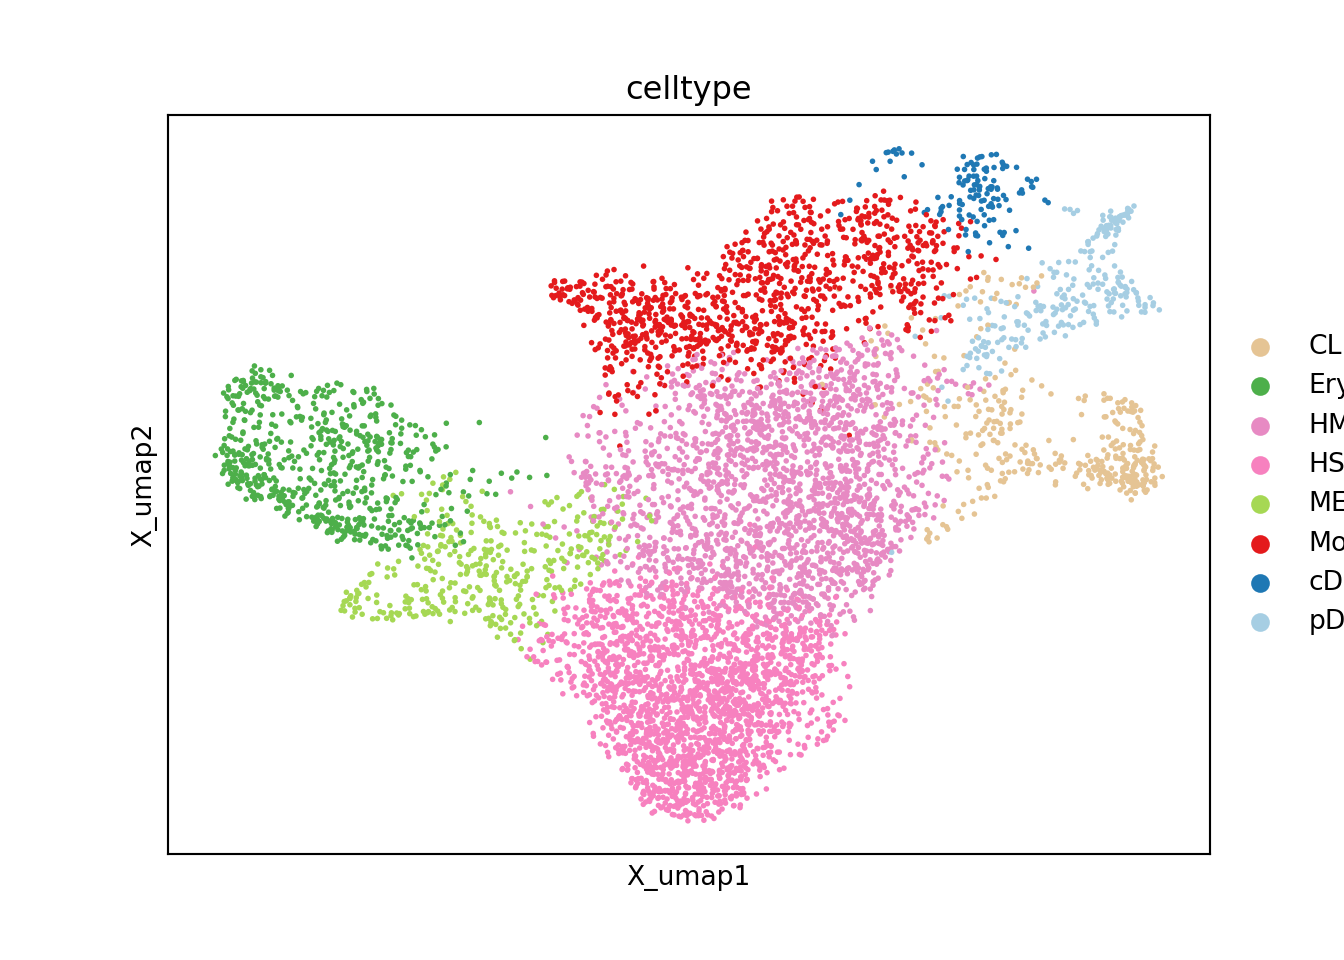
\includegraphics{index_files/figure-latex/unnamed-chunk-6-1.pdf}

\begin{Shaded}
\begin{Highlighting}[]
\NormalTok{directory }\OperatorTok{=}\NormalTok{ os.path.join(}\StringTok{"data"}\NormalTok{, }\StringTok{"3k\_pbmc"}\NormalTok{)}

\ControlFlowTok{if} \KeywordTok{not}\NormalTok{ os.path.exists(directory):}
\NormalTok{    os.makedirs(directory)}
    
\NormalTok{adata.write\_h5ad(os.path.join(}\StringTok{"data"}\NormalTok{, }\StringTok{"3k\_pbmc"}\NormalTok{, }\StringTok{"singlecell\_anndata\_filtered.h5ad"}\NormalTok{))}
\end{Highlighting}
\end{Shaded}

\begin{Shaded}
\begin{Highlighting}[]
\FunctionTok{library}\NormalTok{(reticulate)}
\FunctionTok{library}\NormalTok{(Seurat)}
\CommentTok{\#\textgreater{} Attaching SeuratObject}
\NormalTok{raw\_counts }\OtherTok{\textless{}{-}}\NormalTok{ Matrix}\SpecialCharTok{::}\FunctionTok{t}\NormalTok{(}\FunctionTok{as}\NormalTok{(py}\SpecialCharTok{$}\NormalTok{adata}\SpecialCharTok{$}\NormalTok{raw}\SpecialCharTok{$}\NormalTok{X, }\StringTok{"CsparseMatrix"}\NormalTok{))}
\FunctionTok{colnames}\NormalTok{(raw\_counts) }\OtherTok{\textless{}{-}} \FunctionTok{rownames}\NormalTok{(py}\SpecialCharTok{$}\NormalTok{adata}\SpecialCharTok{$}\NormalTok{obs)}
\FunctionTok{rownames}\NormalTok{(raw\_counts) }\OtherTok{\textless{}{-}} \FunctionTok{rownames}\NormalTok{(py}\SpecialCharTok{$}\NormalTok{adata}\SpecialCharTok{$}\NormalTok{var)}

\CommentTok{\# norm\_counts \textless{}{-} Matrix::t(as(py$ad$X, "CsparseMatrix"))}
\CommentTok{\# colnames(norm\_counts) \textless{}{-} rownames(py$ad$obs)}
\CommentTok{\# rownames(norm\_counts) \textless{}{-} rownames(py$ad$var)}

\NormalTok{pbmc }\OtherTok{\textless{}{-}} \FunctionTok{CreateSeuratObject}\NormalTok{(}\AttributeTok{counts =}\NormalTok{ raw\_counts, }\AttributeTok{meta.data =}\NormalTok{ py}\SpecialCharTok{$}\NormalTok{adata}\SpecialCharTok{$}\NormalTok{obs)}
\CommentTok{\#\textgreater{} Warning: Feature names cannot have underscores (\textquotesingle{}\_\textquotesingle{}), replacing with dashes}
\CommentTok{\#\textgreater{} (\textquotesingle{}{-}\textquotesingle{})}
\CommentTok{\# pbmc@assays$RNA@data \textless{}{-} norm\_counts}
\FunctionTok{saveRDS}\NormalTok{(pbmc, }\AttributeTok{file =} \FunctionTok{paste0}\NormalTok{(}\StringTok{"data/3k\_pbmc/singlecell\_seurat\_filtered.rds"}\NormalTok{))}
\end{Highlighting}
\end{Shaded}

\hypertarget{the-metacell-concept}{%
\chapter{The metacell concept}\label{the-metacell-concept}}

See chapters \ref{MC2}, \ref{SuperCell}, \ref{SEACells}

\hypertarget{MC2}{%
\section{Metacell (MC2)}\label{MC2}}

\hypertarget{SuperCell}{%
\section{SuperCell}\label{SuperCell}}

\hypertarget{SEACells}{%
\section{SEACells}\label{SEACells}}

\hypertarget{constructing-metacells-for-discrete-data}{%
\chapter{Constructing metacells (for `discrete' data)}\label{constructing-metacells-for-discrete-data}}

In this chapter, we will demonstrate metacell construction using three different methods. MetaCell-2 (MC2) and SEACells in Pyhton and SuperCell in R.

For this, we will use a dataset of PBMCs from study. This dataset contains 30K cells and \ldots{} This is an example of a complex dataset with well defined cells types. For an example of more continuous data, see chapter \ref{MC-continuous}

\begin{verbatim}
#> findfont: Font family ['Raleway'] not found. Falling back to DejaVu Sans.
#> findfont: Font family ['Lato'] not found. Falling back to DejaVu Sans.
\end{verbatim}

\hypertarget{mc2-python}{%
\section{MC2 (Python)}\label{mc2-python}}

In this section, we construct metacells using \href{https://github.com/tanaylab/metacells}{Metacell-2 (MC2)}. The code is adapted from the \href{https://metacells.readthedocs.io/en/latest/Metacells_Vignette.html}{author's tutorial}. For more information on the method, please refer to the section 1 of chapter 2.

\hypertarget{importing-python-packages}{%
\subsubsection*{Importing python packages}\label{importing-python-packages}}
\addcontentsline{toc}{subsubsection}{Importing python packages}

To run Metacell-2, the following python packages need to be imported:

\begin{Shaded}
\begin{Highlighting}[]
\ImportTok{import}\NormalTok{ os}
\ImportTok{import}\NormalTok{ numpy }\ImportTok{as}\NormalTok{ np}
\ImportTok{import}\NormalTok{ pandas }\ImportTok{as}\NormalTok{ pd}
\ImportTok{import}\NormalTok{ anndata }\ImportTok{as}\NormalTok{ ad}
\ImportTok{import}\NormalTok{ scanpy }\ImportTok{as}\NormalTok{ sc}
\ImportTok{import}\NormalTok{ matplotlib.pyplot }\ImportTok{as}\NormalTok{ plt}
\ImportTok{import}\NormalTok{ seaborn }\ImportTok{as}\NormalTok{ sns}
\ImportTok{import}\NormalTok{ metacells }\ImportTok{as}\NormalTok{ mc}
\end{Highlighting}
\end{Shaded}

\begin{Shaded}
\begin{Highlighting}[]
\ImportTok{import}\NormalTok{ sys}
\NormalTok{sys.path.append(}\StringTok{\textquotesingle{}./mc\_QC/\textquotesingle{}}\NormalTok{)}
\ImportTok{import}\NormalTok{ mc\_QC}
\end{Highlighting}
\end{Shaded}

If you don't have these packages installed, please refer to the section 2 of chapter 1.

\hypertarget{data-loading}{%
\subsection{Data loading}\label{data-loading}}

We will run Metacell-2 (MC2) on a single-cell dataset composed of XX peripheral blood mononuclear cells (PBMCs). Please follow the section 4 from Chapter 1 to retrieve these data from the scanpy package and save the data in the following file: ``data/3k\_pbmc/singlecell\_anndata\_filtered.h5ad''.

\begin{Shaded}
\begin{Highlighting}[]
\NormalTok{MC\_tool }\OperatorTok{=} \StringTok{"MC2"}
\NormalTok{proj\_name }\OperatorTok{=} \StringTok{"3k\_pbmc"}
\NormalTok{ad }\OperatorTok{=}\NormalTok{ sc.read(os.path.join(}\StringTok{"data"}\NormalTok{, proj\_name, }\StringTok{"singlecell\_anndata\_filtered.h5ad"}\NormalTok{))}
\end{Highlighting}
\end{Shaded}

We initialize the name of the anndata (in the unstructured annotations) object using the \texttt{mc.ut.set\_name()} function from the MC2 package.

\begin{Shaded}
\begin{Highlighting}[]
\NormalTok{mc.ut.set\_name(ad, proj\_name)}
\end{Highlighting}
\end{Shaded}

\hypertarget{filtering-steps}{%
\subsection{Filtering steps}\label{filtering-steps}}

MC2 requires that standard filtering steps such as doublet filtering is performed outside of the MC2 framework.
In addition to standard data filtering steps, the MC2 package proposes functions to filter the single-cell data at the gene and at the cell level (See \href{https://tanaylab.github.io/metacells-vignettes/one-pass.html}{original vignette}).
At the gene level, the filtering steps consist in excluding genes based on biological knowledge (\emph{e.g.} mitochrondrial genes) as well as based on their expression levels.
The latter genes include genes with zero expression or low expression levels and ``bursty lonely genes'' (\emph{i.e.}, genes with high expression levels but no correlation with any other gene).
At the cell level, filtering is performed based on cells UMI counts.

\hypertarget{gene-filtering}{%
\subsubsection*{Gene filtering}\label{gene-filtering}}
\addcontentsline{toc}{subsubsection}{Gene filtering}

In section XX form Chapter XX, we pre-processed the raw scRNA-Seq data and excluded genes with low expression as well as mitochondrial genes.
In the following code chunk, we exclude additional genes using the \texttt{mc.pl.exclude\_genes()}function from the MC2 package.
Based on the authors vignette, we provide a minimal list of genes to exclude, \emph{i.e.}, sex-specific and non-coding genes. To complete this list of genes, an iterative approach can be used following the guidelines of the MC2 authors in a \href{https://tanaylab.github.io/metacells-vignettes/iterative.html}{second vignette}.
The \texttt{mc.pl.exclude\_genes()}function will filter out: i) the known-to-be-excluded genes defined by the user as gene names or gene names patterns (\texttt{EXCLUDED\_GENE\_NAMES} and \texttt{EXCLUDED\_GENE\_PATTERNS} parameters respectively),
and ii) the ``bursty lonely genes''.

\begin{Shaded}
\begin{Highlighting}[]
\NormalTok{EXCLUDED\_GENE\_NAMES }\OperatorTok{=}\NormalTok{ [}\StringTok{"XIST"}\NormalTok{, }\StringTok{"MALAT1"}\NormalTok{, }\StringTok{"NEAT1"}\NormalTok{] }
\NormalTok{EXCLUDED\_GENE\_PATTERNS }\OperatorTok{=}\NormalTok{ [}\StringTok{\textquotesingle{}MT{-}.*\textquotesingle{}}\NormalTok{]}

\NormalTok{mc.pl.exclude\_genes(}
\NormalTok{    ad,}
\NormalTok{    excluded\_gene\_names}\OperatorTok{=}\NormalTok{EXCLUDED\_GENE\_NAMES, }
\NormalTok{    excluded\_gene\_patterns}\OperatorTok{=}\NormalTok{EXCLUDED\_GENE\_PATTERNS,}
\NormalTok{    random\_seed}\OperatorTok{=}\DecValTok{123456}\NormalTok{,}
\NormalTok{)}
\CommentTok{\#\textgreater{} set 3k\_pbmc.var[bursty\_lonely\_gene]: 0 true (0\%) out of 32738 bools}
\CommentTok{\#\textgreater{} set 3k\_pbmc.var[properly\_sampled\_gene]: 16579 true (50.64\%) out of 32738 bools}
\CommentTok{\#\textgreater{} set 3k\_pbmc.var[excluded\_gene]: 16174 true (49.4\%) out of 32738 bools}
\end{Highlighting}
\end{Shaded}

\hypertarget{cell-filtering-based-on-umis-counts}{%
\subsubsection*{Cell filtering based on UMIs counts}\label{cell-filtering-based-on-umis-counts}}
\addcontentsline{toc}{subsubsection}{Cell filtering based on UMIs counts}

In the MC2 framework, cells with very low and very high UMI content will be filtered out (\texttt{PROPERLY\_SAMPLED\_MIN\_CELL\_TOTAL}, \texttt{PROPERLY\_SAMPLED\_MAX\_CELL\_TOTAL} variables defining thresholds in the next code chunk).\\
Also, cell filtering based on UMI counts in excluded genes is also performed(\texttt{PROPERLY\_SAMPLED\_MAX\_EXCLUDED\_GENES\_FRACTION} variable).
Since our dataset has been pre-filtered, very lenient cutoffs will be used in this tutorial.
The following code chunk defines these parameters. To adapt them to your datasets, we advise you to explore the distributions of total UMI counts and UMI counts in excluded genes, as recommended and described in the MC2 \href{https://tanaylab.github.io/metacells-vignettes/one-pass.html}{original vignette}.

\begin{Shaded}
\begin{Highlighting}[]
\NormalTok{PROPERLY\_SAMPLED\_MIN\_CELL\_TOTAL }\OperatorTok{=} \DecValTok{200} 
\NormalTok{PROPERLY\_SAMPLED\_MAX\_CELL\_TOTAL }\OperatorTok{=} \DecValTok{10000} 
\NormalTok{PROPERLY\_SAMPLED\_MAX\_EXCLUDED\_GENES\_FRACTION }\OperatorTok{=} \FloatTok{0.25}
\end{Highlighting}
\end{Shaded}

The number of UMIs in excluded genes is computed using the \texttt{mc.tl.compute\_excluded\_gene\_umis()} function and cells are filtered out using the \texttt{mc.pl.exclude\_cells()} function.
Additional cells can be filtered out by adding a cell description columns in the \texttt{obs} data frame in the anndata oject. This annotation should be a boolean indicating whether the cell should filtered out or not.
The name of this column should be provided to the \texttt{mc.pl.exclude\_cells()} function via the \texttt{additional\_cells\_masks} parameter.

\begin{Shaded}
\begin{Highlighting}[]
\NormalTok{mc.tl.compute\_excluded\_gene\_umis(ad)}

\NormalTok{mc.pl.exclude\_cells(}
\NormalTok{    ad,}
\NormalTok{    properly\_sampled\_min\_cell\_total}\OperatorTok{=}\NormalTok{PROPERLY\_SAMPLED\_MIN\_CELL\_TOTAL,}
\NormalTok{    properly\_sampled\_max\_cell\_total}\OperatorTok{=}\NormalTok{PROPERLY\_SAMPLED\_MAX\_CELL\_TOTAL,}
\NormalTok{    properly\_sampled\_max\_excluded\_genes\_fraction}\OperatorTok{=}\NormalTok{PROPERLY\_SAMPLED\_MAX\_EXCLUDED\_GENES\_FRACTION }\CommentTok{\# ,}
    \CommentTok{\# additional\_cells\_masks=["|doublet\_cell"]}
\NormalTok{)}
\CommentTok{\#\textgreater{} set 3k\_pbmc.obs[properly\_sampled\_cell]: 2638 true (100\%) out of 2638 bools}
\CommentTok{\#\textgreater{} set 3k\_pbmc.obs[excluded\_cell]: 0 true (0\%) out of 2638 bools}
\end{Highlighting}
\end{Shaded}

After performing the two-step filtering (genes and cells), the ``cleaned'' data can be extracted using the \texttt{mc.pl.extract\_clean\_data()} function.

\begin{Shaded}
\begin{Highlighting}[]
\CommentTok{\# Extract clean dataset (with filtered cells and genes)}
\NormalTok{ad }\OperatorTok{=}\NormalTok{ mc.pl.extract\_clean\_data(ad)}
\CommentTok{\#\textgreater{} set 3k\_pbmc.clean.obs[full\_cell\_index]: 2638 int32s}
\CommentTok{\#\textgreater{} set 3k\_pbmc.clean.var[full\_gene\_index]: 16564 int32s}
\end{Highlighting}
\end{Shaded}

\hypertarget{building-metacells}{%
\subsection{Building metacells}\label{building-metacells}}

\hypertarget{defining-lateral-genes}{%
\subsubsection*{Defining lateral genes}\label{defining-lateral-genes}}
\addcontentsline{toc}{subsubsection}{Defining lateral genes}

To build metacells, we need to define lateral genes, which are genes with strong biological signal which is independent of cell-state, \emph{e.g.} cell-cycle genes.
These genes will be ignored for computing cells similarity and build metacells
but will be considered to define outlier cells (\emph{i.e.}, expression levels of lateral genes should be consistent within metacells).
In the following chunk, we consider a minimal list of lateral genes including cell-cycle and ribosomal genes and mark them in the MC2 object using the \texttt{mc.pl.mark\_lateral\_genes()} function.

\begin{Shaded}
\begin{Highlighting}[]

\NormalTok{LATERAL\_GENE\_NAMES }\OperatorTok{=}\NormalTok{ [}
    \StringTok{"AURKA"}\NormalTok{, }\StringTok{"MCM3"}\NormalTok{, }\StringTok{"MCM4"}\NormalTok{, }\StringTok{"MCM7"}\NormalTok{, }\StringTok{"MKI67"}\NormalTok{, }\StringTok{"PCNA"}\NormalTok{, }\StringTok{"RRM2"}\NormalTok{, }\StringTok{"SMC4"}\NormalTok{, }\StringTok{"TPX2"}\NormalTok{,  }\CommentTok{\# Cell{-}cycle}
    \StringTok{"FOS"}\NormalTok{, }\StringTok{"HSP90AB1"}\NormalTok{, }\StringTok{"TXN"}\NormalTok{,                                                  }\CommentTok{\# Stress}
\NormalTok{]}
\NormalTok{LATERAL\_GENE\_PATTERNS }\OperatorTok{=}\NormalTok{ [}\StringTok{"RP[LS].*"}\NormalTok{]  }\CommentTok{\# Ribosomal}

\CommentTok{\# This will mark as "lateral\_gene" any genes that match the above, if they exist in the clean dataset.}
\NormalTok{mc.pl.mark\_lateral\_genes(}
\NormalTok{    ad,}
\NormalTok{    lateral\_gene\_names}\OperatorTok{=}\NormalTok{LATERAL\_GENE\_NAMES,}
\NormalTok{    lateral\_gene\_patterns}\OperatorTok{=}\NormalTok{LATERAL\_GENE\_PATTERNS,}
\NormalTok{)}
\CommentTok{\#\textgreater{} set 3k\_pbmc.clean.var[lateral\_gene]: 111 true (0.6701\%) out of 16564 bools}
\end{Highlighting}
\end{Shaded}

Some genes have higher variances that expected which could lead to false positive outlier identification.
Users can mark those genes as \emph{noisy genes} using the \texttt{mc.pl.mark\_noisy\_genes()} function.

\begin{Shaded}
\begin{Highlighting}[]

\NormalTok{NOISY\_GENE\_NAMES }\OperatorTok{=}\NormalTok{ [}
    \StringTok{"CCL3"}\NormalTok{, }\StringTok{"CCL4"}\NormalTok{, }\StringTok{"CCL5"}\NormalTok{, }\StringTok{"CXCL8"}\NormalTok{, }\StringTok{"DUSP1"}\NormalTok{, }\StringTok{"FOS"}\NormalTok{, }\StringTok{"G0S2"}\NormalTok{, }\StringTok{"HBB"}\NormalTok{, }\StringTok{"HIST1H4C"}\NormalTok{, }\StringTok{"IER2"}\NormalTok{, }\StringTok{"IGKC"}\NormalTok{,}
    \StringTok{"IGLC2"}\NormalTok{, }\StringTok{"JUN"}\NormalTok{, }\StringTok{"JUNB"}\NormalTok{, }\StringTok{"KLRB1"}\NormalTok{, }\StringTok{"MT2A"}\NormalTok{, }\StringTok{"RPS26"}\NormalTok{, }\StringTok{"RPS4Y1"}\NormalTok{, }\StringTok{"TRBC1"}\NormalTok{, }\StringTok{"TUBA1B"}\NormalTok{, }\StringTok{"TUBB"}
\NormalTok{]}
\CommentTok{\# This will mark as "noisy\_gene" any genes that match the above, if they exist in the clean dataset.}
\NormalTok{mc.pl.mark\_noisy\_genes(ad, noisy\_gene\_names}\OperatorTok{=}\NormalTok{NOISY\_GENE\_NAMES)}
\CommentTok{\#\textgreater{} set 3k\_pbmc.clean.var[noisy\_gene]: 17 true (0.1026\%) out of 16564 bools}
\end{Highlighting}
\end{Shaded}

To extend this list of lateral genes, users can use the `` function to identify genes that are highly correlated with the predefined lateral genes.

\hypertarget{estimate-target_metacell_size-gamma}{%
\subsubsection*{Estimate target\_metacell\_size (gamma)}\label{estimate-target_metacell_size-gamma}}
\addcontentsline{toc}{subsubsection}{Estimate target\_metacell\_size (gamma)}

By default, MC2 will build metacells with a size of 96 cells per metacells.
Users can vary the \texttt{target\_metacell\_size} parameter to reach a desired graining level.

\begin{Shaded}
\begin{Highlighting}[]
\NormalTok{gamma   }\OperatorTok{=} \DecValTok{50} \CommentTok{\# graining level}

\NormalTok{target\_metacell\_size }\OperatorTok{=} \BuiltInTok{round}\NormalTok{(ad.shape[}\DecValTok{0}\NormalTok{]}\OperatorTok{/}\NormalTok{gamma)}
\NormalTok{target\_metacell\_size}
\CommentTok{\#\textgreater{} 53}
\end{Highlighting}
\end{Shaded}

\hypertarget{metacells-identification-using-the-divide-and-conquer-approach}{%
\subsubsection*{Metacells identification using the divide and conquer approach}\label{metacells-identification-using-the-divide-and-conquer-approach}}
\addcontentsline{toc}{subsubsection}{Metacells identification using the divide and conquer approach}

The construction of metacells by MC2 is performed using the \texttt{mc.pl.divide\_and\_conquer\_pipeline()} function.
Note that by default all cores of the system will be used for the metacells construction.
To change this behavior and adapt the number of cores the MC2 authors propose to use the \texttt{mc.pl.guess\_max\_parallel\_piles()} and \texttt{mc.pl.set\_max\_parallel\_piles()} functions to adapt the number of processed in parallel depending on the available memory.

\begin{Shaded}
\begin{Highlighting}[]
\NormalTok{max\_parallel\_piles }\OperatorTok{=}\NormalTok{ mc.pl.guess\_max\_parallel\_piles(ad)}
\NormalTok{mc.pl.set\_max\_parallel\_piles(max\_parallel\_piles)}
\NormalTok{mc.pl.divide\_and\_conquer\_pipeline(}
\NormalTok{    ad,}
\NormalTok{    target\_metacell\_size }\OperatorTok{=}\NormalTok{ target\_metacell\_size,}
\NormalTok{    random\_seed }\OperatorTok{=} \DecValTok{123456}\NormalTok{)}
\CommentTok{\#\textgreater{} set 3k\_pbmc.clean.var[selected\_gene]: * {-}\textgreater{} False}
\CommentTok{\#\textgreater{} set 3k\_pbmc.clean.var[rare\_gene]: 0 true (0\%) out of 16564 bools}
\CommentTok{\#\textgreater{} set 3k\_pbmc.clean.var[rare\_gene\_module]: 16564 int32 elements with all outliers (100\%)}
\CommentTok{\#\textgreater{} set 3k\_pbmc.clean.obs[cells\_rare\_gene\_module]: 2638 int32 elements with all outliers (100\%)}
\CommentTok{\#\textgreater{} set 3k\_pbmc.clean.obs[rare\_cell]: 0 true (0\%) out of 2638 bools}
\CommentTok{\#\textgreater{} set 3k\_pbmc.clean.var[selected\_gene]: 295 true (1.781\%) out of 16564 bools}
\CommentTok{\#\textgreater{} set 3k\_pbmc.clean.obs[metacell]: 2638 int32s}
\CommentTok{\#\textgreater{} set 3k\_pbmc.clean.obs[dissolved]: 14 true (0.5307\%) out of 2638 bools}
\CommentTok{\#\textgreater{} set 3k\_pbmc.clean.obs[metacell\_level]: 2638 int32s}

\NormalTok{ad.obs.metacell.head}
\CommentTok{\#\textgreater{} \textless{}bound method NDFrame.head of index}
\CommentTok{\#\textgreater{} AAACATACAACCAC{-}1    30}
\CommentTok{\#\textgreater{} AAACATTGAGCTAC{-}1    31}
\CommentTok{\#\textgreater{} AAACATTGATCAGC{-}1    49}
\CommentTok{\#\textgreater{} AAACCGTGCTTCCG{-}1    13}
\CommentTok{\#\textgreater{} AAACCGTGTATGCG{-}1    {-}1}
\CommentTok{\#\textgreater{}                     ..}
\CommentTok{\#\textgreater{} TTTCGAACTCTCAT{-}1    43}
\CommentTok{\#\textgreater{} TTTCTACTGAGGCA{-}1    25}
\CommentTok{\#\textgreater{} TTTCTACTTCCTCG{-}1    57}
\CommentTok{\#\textgreater{} TTTGCATGAGAGGC{-}1    16}
\CommentTok{\#\textgreater{} TTTGCATGCCTCAC{-}1    49}
\CommentTok{\#\textgreater{} Name: metacell, Length: 2638, dtype: int32\textgreater{}}
\end{Highlighting}
\end{Shaded}

\hypertarget{retrieve-aggregated-metacell-data}{%
\subsubsection*{Retrieve aggregated metacell data}\label{retrieve-aggregated-metacell-data}}
\addcontentsline{toc}{subsubsection}{Retrieve aggregated metacell data}

The \texttt{mc.pl.divide\_and\_conquer\_pipeline()} function associates each cell to a metacell or defines the cell as outlier. These assignments are found in the \texttt{obs} layer of the anndata object
The function \texttt{pl.collect\_metacells} should be used to subsequently retrieve an anndata object containing the data at the metacells level instead of the single-cell level.

\begin{Shaded}
\begin{Highlighting}[]

\NormalTok{mc\_ad }\OperatorTok{=}\NormalTok{ mc.pl.collect\_metacells(ad, name}\OperatorTok{=}\StringTok{\textquotesingle{}metacells\textquotesingle{}}\NormalTok{, random\_seed }\OperatorTok{=} \DecValTok{123456}\NormalTok{)}
\CommentTok{\#\textgreater{} set metacells.obs[grouped]: 62 int64s}
\CommentTok{\#\textgreater{} set metacells.obs[total\_umis]: 62 float64s}
\CommentTok{\#\textgreater{} set metacells.layers[total\_umis]: ndarray 62 X 16564 float32s}
\CommentTok{\#\textgreater{} set metacells.obs[\_\_zeros\_downsample\_umis]: 62 int64s}
\CommentTok{\#\textgreater{} set metacells.layers[zeros]: ndarray 62 X 16564 int32s}
\CommentTok{\#\textgreater{} set 3k\_pbmc.clean.obs[metacell\_name]: 2638 \textless{}U8s}
\CommentTok{\#\textgreater{} set metacells.var[gene\_ids]: 16564 objects}
\CommentTok{\#\textgreater{} set metacells.var[bursty\_lonely\_gene]: 0 true (0\%) out of 16564 bools}
\CommentTok{\#\textgreater{} set metacells.var[properly\_sampled\_gene]: 16564 true (100\%) out of 16564 bools}
\CommentTok{\#\textgreater{} set metacells.var[excluded\_gene]: 0 true (0\%) out of 16564 bools}
\CommentTok{\#\textgreater{} set metacells.var[full\_gene\_index]: 16564 int32s}
\CommentTok{\#\textgreater{} set metacells.var[lateral\_gene]: 111 true (0.6701\%) out of 16564 bools}
\CommentTok{\#\textgreater{} set metacells.var[noisy\_gene]: 17 true (0.1026\%) out of 16564 bools}
\CommentTok{\#\textgreater{} set metacells.var[selected\_gene]: 295 true (1.781\%) out of 16564 bools}
\CommentTok{\#\textgreater{} set metacells.var[rare\_gene]: 0 true (0\%) out of 16564 bools}
\CommentTok{\#\textgreater{} set metacells.var[rare\_gene\_module]: 16564 int32s}
\CommentTok{\#\textgreater{} set metacells.obs[metacells\_rare\_gene\_module]: 62 int32s}
\CommentTok{\#\textgreater{} set metacells.obs[rare\_metacell]: 0 true (0\%) out of 62 bools}
\CommentTok{\#\textgreater{} set metacells.uns[outliers]: 158}
\CommentTok{\#\textgreater{} set metacells.uns[metacells\_algorithm]: metacells.0.9.0}
\NormalTok{mc\_ad.shape}
\CommentTok{\#\textgreater{} (62, 16564)}
\end{Highlighting}
\end{Shaded}

\textbf{Comparing the obtained and requested graining level}

In the following code chunk, we estimate whether a deviation of the obtained gamma from the requested gamma is acceptable. If not, we suggest to increase or decrease the \texttt{target\_metacell\_size} parameter to approach the desired graining level.

\begin{Shaded}
\begin{Highlighting}[]
\NormalTok{gamma\_obtained }\OperatorTok{=}\NormalTok{ ad.shape[}\DecValTok{0}\NormalTok{]}\OperatorTok{/}\NormalTok{mc\_ad.shape[}\DecValTok{0}\NormalTok{]}
\BuiltInTok{print}\NormalTok{(gamma\_obtained)}
\CommentTok{\#\textgreater{} 42.54838709677419}

\NormalTok{gamma\_dev }\OperatorTok{=}\NormalTok{ (gamma\_obtained }\OperatorTok{{-}}\NormalTok{ gamma)}\OperatorTok{/}\NormalTok{gamma}
\ControlFlowTok{if} \BuiltInTok{abs}\NormalTok{(gamma\_dev) }\OperatorTok{\textless{}} \FloatTok{0.3}\NormalTok{: }
\NormalTok{    gamma\_dev }\OperatorTok{=} \DecValTok{0}

\ControlFlowTok{if}\NormalTok{ gamma\_dev }\OperatorTok{\textless{}} \DecValTok{0}\NormalTok{:}
    \BuiltInTok{print}\NormalTok{(}\StringTok{"Increase \textasciigrave{}target\_metacell\_size\textasciigrave{} parameter by increasing \textasciigrave{}scale\textasciigrave{} and re{-}run metacell divide\_and\_conquer\_pipeline() to get larger graining level"}\NormalTok{)}
\ControlFlowTok{elif}\NormalTok{ gamma\_dev }\OperatorTok{\textgreater{}} \DecValTok{0}\NormalTok{:}
    \BuiltInTok{print}\NormalTok{(}\StringTok{"Deacrease \textasciigrave{}target\_metacell\_size\textasciigrave{} parameter by decreasing \textasciigrave{}scale\textasciigrave{} and re{-}run metacell divide\_and\_conquer\_pipeline() to get smaller graining level"}\NormalTok{)}
\ControlFlowTok{elif}\NormalTok{ gamma\_dev }\OperatorTok{==} \DecValTok{0}\NormalTok{:}
    \BuiltInTok{print}\NormalTok{(}\StringTok{"The obtained graining level is acceptable, no need to re{-}run the metacell divide\_and\_conquer\_pipeline() with a new \textasciigrave{}target\_metacell\_size\textasciigrave{} "}\NormalTok{)}
\CommentTok{\#\textgreater{} The obtained graining level is acceptable, no need to re{-}run the metacell divide\_and\_conquer\_pipeline() with a new \textasciigrave{}target\_metacell\_size\textasciigrave{}}
\end{Highlighting}
\end{Shaded}

\hypertarget{visualize-metacells}{%
\subsection{Visualize metacells}\label{visualize-metacells}}

If single-cell annotations are available in the original single-cell anndata object. We can transfer these annotations to the metacell anndata object
using the \texttt{mc.tl.convey\_obs\_to\_group()} function which will associate each metacell to the most frequent annotation (categorical) or averaged annotation (continuous) across the single-cells composing the metacell
(use of the \texttt{mc.ut.most\_frequent} and \texttt{np.mean} respectively in the \texttt{mode} paratemer).

\begin{Shaded}
\begin{Highlighting}[]
\CommentTok{\# Assign a single value for each metacell based on the cells.}
\NormalTok{mc.tl.convey\_obs\_to\_group(}
\NormalTok{    adata}\OperatorTok{=}\NormalTok{ad, gdata}\OperatorTok{=}\NormalTok{mc\_ad,}
\NormalTok{    property\_name}\OperatorTok{=}\StringTok{"louvain"}\NormalTok{, to\_property\_name}\OperatorTok{=}\StringTok{"annotation"}\NormalTok{,}
\NormalTok{    method}\OperatorTok{=}\NormalTok{mc.ut.most\_frequent  }\CommentTok{\# This is the default, for categorical data}
\NormalTok{)}
\CommentTok{\#\textgreater{} set metacells.obs[annotation]: 62 \textless{}U17s}

\CommentTok{\# Compute the fraction of cells with each possible value in each metacell:}
\NormalTok{mc.tl.convey\_obs\_fractions\_to\_group(  }
\NormalTok{    adata}\OperatorTok{=}\NormalTok{ad, gdata}\OperatorTok{=}\NormalTok{mc\_ad,}
\NormalTok{    property\_name}\OperatorTok{=}\StringTok{"louvain"}\NormalTok{, to\_property\_name}\OperatorTok{=}\StringTok{"annotation"}
\NormalTok{)}
\CommentTok{\#\textgreater{} set metacells.obs[annotation\_fraction\_of\_B cells]: 62 float64s}
\CommentTok{\#\textgreater{} set metacells.obs[annotation\_fraction\_of\_CD14+ Monocytes]: 62 float64s}
\CommentTok{\#\textgreater{} set metacells.obs[annotation\_fraction\_of\_CD4 T cells]: 62 float64s}
\CommentTok{\#\textgreater{} set metacells.obs[annotation\_fraction\_of\_CD8 T cells]: 62 float64s}
\CommentTok{\#\textgreater{} set metacells.obs[annotation\_fraction\_of\_Dendritic cells]: 62 float64s}
\CommentTok{\#\textgreater{} set metacells.obs[annotation\_fraction\_of\_FCGR3A+ Monocytes]: 62 float64s}
\CommentTok{\#\textgreater{} set metacells.obs[annotation\_fraction\_of\_Megakaryocytes]: 62 float64s}
\CommentTok{\#\textgreater{} set metacells.obs[annotation\_fraction\_of\_NK cells]: 62 float64s}
\end{Highlighting}
\end{Shaded}

The following code chunk adds a columns named \texttt{membership} and containing the single\_cell assignments to the obs attribute in the anndata object containing the raw data.
This annotation will be used in the mc\_QC package to compute metacells quality metrics. We also save the single-cell metadata in the metacell anndata object.

\begin{Shaded}
\begin{Highlighting}[]
\CommentTok{\# make a membership {-}{-} index of metacells to which single cells belong to }
\NormalTok{ad.obs[}\StringTok{\textquotesingle{}membership\textquotesingle{}}\NormalTok{] }\OperatorTok{=}\NormalTok{ [}\BuiltInTok{int}\NormalTok{(i)}\OperatorTok{+}\DecValTok{1} \ControlFlowTok{if}\NormalTok{ i }\OperatorTok{\textgreater{}=} \DecValTok{0} \ControlFlowTok{else}\NormalTok{ np.nan }\ControlFlowTok{for}\NormalTok{ i }\KeywordTok{in}\NormalTok{ ad.obs.metacell] }

\CommentTok{\#\# Save single{-}cell metadata (i.e., \textasciigrave{}raw.obs\textasciigrave{} dataframe) in the metacell adata object}
\NormalTok{mc\_ad.uns }\OperatorTok{=}\NormalTok{ ad.uns.copy()}
\NormalTok{mc\_ad.uns[}\StringTok{\textquotesingle{}sc.obs\textquotesingle{}}\NormalTok{] }\OperatorTok{=}\NormalTok{ ad.obs.copy()}

\CommentTok{\# save the requested gamma}
\NormalTok{mc\_ad.uns[}\StringTok{\textquotesingle{}gamma\textquotesingle{}}\NormalTok{] }\OperatorTok{=}\NormalTok{ gamma}
\end{Highlighting}
\end{Shaded}

\hypertarget{compute-latent-space-for-metacell-qc}{%
\subsubsection*{Compute latent space for metacell QC}\label{compute-latent-space-for-metacell-qc}}
\addcontentsline{toc}{subsubsection}{Compute latent space for metacell QC}

To visualize the metacells, we can project the metacells on the single-cell UMAP representation. To run UMAP, we will generate in the next code chunk a lower-dimentional embedding of the data, so far not needed since the MC2 methods builds metacells from gene expression data and not from latent space.
Also, note that some of the QC metrics (e.g., \textbf{compactness} and \textbf{separation}), that we will compute in the next section of this tutorial, are computed from this latent space.

\begin{Shaded}
\begin{Highlighting}[]
\CommentTok{\# Save count as a separate layer}
\NormalTok{ad.layers[}\StringTok{\textquotesingle{}counts\textquotesingle{}}\NormalTok{] }\OperatorTok{=}\NormalTok{ ad.X}

\CommentTok{\# Copy the counts to ".raw" attribute of the anndata since it is necessary for downstream analysis}
\CommentTok{\# This step should be performed after filtering }
\NormalTok{raw\_ad }\OperatorTok{=}\NormalTok{ sc.AnnData(ad.layers[}\StringTok{\textquotesingle{}counts\textquotesingle{}}\NormalTok{])}
\NormalTok{raw\_ad.obs\_names, raw\_ad.var\_names }\OperatorTok{=}\NormalTok{ ad.obs\_names, ad.var\_names}
\NormalTok{ad.raw }\OperatorTok{=}\NormalTok{ raw\_ad}


\CommentTok{\# Normalize cells, log transform and compute highly variable genes}
\NormalTok{sc.pp.normalize\_per\_cell(ad)}
\NormalTok{sc.pp.log1p(ad)}
\NormalTok{sc.pp.highly\_variable\_genes(ad, n\_top\_genes}\OperatorTok{=}\DecValTok{1000}\NormalTok{)}

\CommentTok{\# Compute principal components {-} }

\NormalTok{n\_comp    }\OperatorTok{=} \DecValTok{10}
\NormalTok{sc.tl.pca(ad, n\_comps}\OperatorTok{=}\NormalTok{n\_comp, use\_highly\_variable}\OperatorTok{=}\VariableTok{True}\NormalTok{)}


\CommentTok{\# Compute UMAP for visualization }
\NormalTok{sc.pp.neighbors(ad, n\_neighbors}\OperatorTok{=}\DecValTok{10}\NormalTok{, n\_pcs}\OperatorTok{=}\NormalTok{n\_comp)}
\NormalTok{sc.tl.umap(ad)}
\end{Highlighting}
\end{Shaded}

To visualize the metacell projection on the single-cell UMAP, we use the \texttt{mc\_visualize} function from the \texttt{mc\_QC}, this function was adapted from the \texttt{plot.plot\_2D} included in the SEACells package.

\begin{Shaded}
\begin{Highlighting}[]
\NormalTok{mc\_proj }\OperatorTok{=}\NormalTok{ mc\_QC.mc\_visualize(ad, key}\OperatorTok{=}\StringTok{\textquotesingle{}X\_umap\textquotesingle{}}\NormalTok{, group\_by\_name}\OperatorTok{=}\StringTok{\textquotesingle{}membership\textquotesingle{}}\NormalTok{, colour\_sc\_name}\OperatorTok{=}\StringTok{\textquotesingle{}louvain\textquotesingle{}}\NormalTok{,  colour\_mc\_name}\OperatorTok{=}\StringTok{\textquotesingle{}membership\textquotesingle{}}\NormalTok{, colour\_metacells}\OperatorTok{=}\VariableTok{True}\NormalTok{, legend\_sc}\OperatorTok{=}\VariableTok{None}\NormalTok{, legend\_mc}\OperatorTok{=}\VariableTok{None}\NormalTok{)}
\CommentTok{\#\textgreater{} No artists with labels found to put in legend.  Note that artists whose label start with an underscore are ignored when legend() is called with no argument.}
\NormalTok{mc\_proj.show()}
\CommentTok{\#\textgreater{} findfont: Font family \textquotesingle{}Bitstream Vera Sans\textquotesingle{} not found.}
\CommentTok{\#\textgreater{} findfont: Font family \textquotesingle{}Bitstream Vera Sans\textquotesingle{} not found.}
\CommentTok{\#\textgreater{} findfont: Font family \textquotesingle{}Bitstream Vera Sans\textquotesingle{} not found.}
\CommentTok{\#\textgreater{} findfont: Font family \textquotesingle{}Bitstream Vera Sans\textquotesingle{} not found.}
\CommentTok{\#\textgreater{} findfont: Font family \textquotesingle{}Bitstream Vera Sans\textquotesingle{} not found.}
\CommentTok{\#\textgreater{} findfont: Font family \textquotesingle{}Bitstream Vera Sans\textquotesingle{} not found.}
\CommentTok{\#\textgreater{} findfont: Font family \textquotesingle{}Bitstream Vera Sans\textquotesingle{} not found.}
\CommentTok{\#\textgreater{} findfont: Font family \textquotesingle{}Bitstream Vera Sans\textquotesingle{} not found.}
\CommentTok{\#\textgreater{} findfont: Font family \textquotesingle{}Bitstream Vera Sans\textquotesingle{} not found.}
\end{Highlighting}
\end{Shaded}

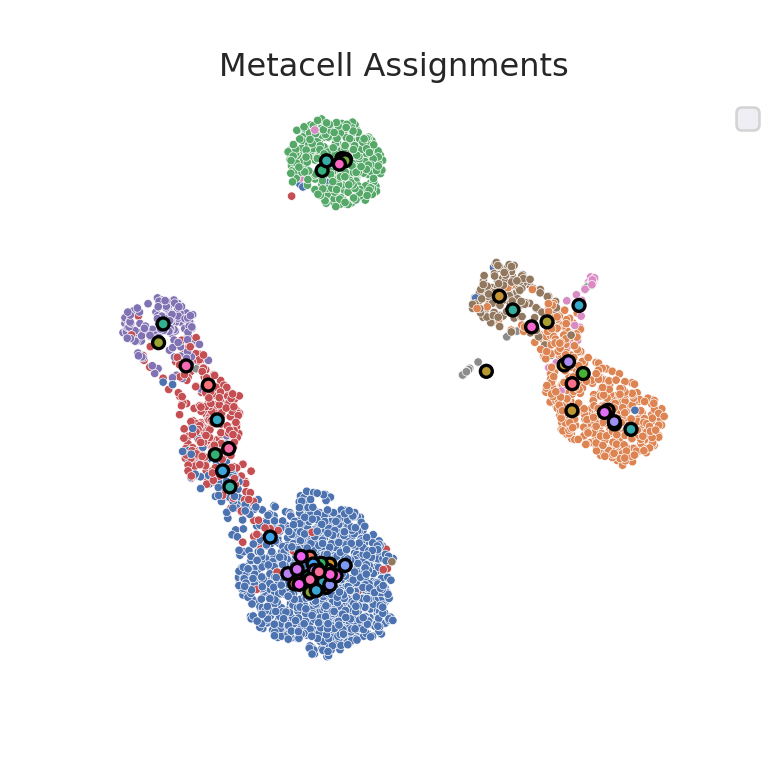
\includegraphics{21-MC_construction_discrete_files/figure-latex/mc2-comp-umap-1.pdf}

\hypertarget{metacell-qc}{%
\subsection{Metacell QC}\label{metacell-qc}}

\hypertarget{compute-purity-compactness-and-separation-metrics}{%
\subsubsection*{Compute purity, compactness and separation metrics}\label{compute-purity-compactness-and-separation-metrics}}
\addcontentsline{toc}{subsubsection}{Compute purity, compactness and separation metrics}

\textbf{Size distribution}

\begin{Shaded}
\begin{Highlighting}[]
\CommentTok{\#mc\_size = SEACells.plot.plot\_SEACell\_sizes(ad, bins=20)}

\CommentTok{\#mc\_ad.obs = pd.merge(mc\_ad.obs, mc\_size, left\_index=True, right\_index=True)}
\CommentTok{\#mc\_ad.obs}
\end{Highlighting}
\end{Shaded}

When available, we can use cell annotation to annotate each metacell to the most abundant cell category (\emph{e.g.} cell type) composing the metacell.
This also allows us to compute metacell purity. If the annotation considered is the cell type, the \textbf{purity} of a metacell is the proportion of the most abundant cell type within the metacell {[}ref SuperCell{]}

\begin{Shaded}
\begin{Highlighting}[]
\NormalTok{mc\_purity }\OperatorTok{=}\NormalTok{ mc\_QC.purity(ad, annotation\_label, MC\_label }\OperatorTok{=} \StringTok{\textquotesingle{}membership\textquotesingle{}}\NormalTok{)}
\NormalTok{mc\_purity.head()}
\CommentTok{\#\textgreater{}                     louvain  louvain\_purity}
\CommentTok{\#\textgreater{} membership                                 }
\CommentTok{\#\textgreater{} 1.0         CD14+ Monocytes        1.000000}
\CommentTok{\#\textgreater{} 2.0             CD8 T cells        0.884058}
\CommentTok{\#\textgreater{} 3.0             CD4 T cells        0.897436}
\CommentTok{\#\textgreater{} 4.0         CD14+ Monocytes        1.000000}
\CommentTok{\#\textgreater{} 5.0             CD4 T cells        1.000000}
\CommentTok{\# add purity to metadata}
\NormalTok{mc\_ad.obs[}\StringTok{\textquotesingle{}purity\textquotesingle{}}\NormalTok{] }\OperatorTok{=} \BuiltInTok{list}\NormalTok{(mc\_purity[annotation\_label }\OperatorTok{+} \StringTok{"\_purity"}\NormalTok{])}
\end{Highlighting}
\end{Shaded}

The \textbf{compactness} of a metacell is the variance of the components within the metacell {[}ref SEACells{]}

\begin{Shaded}
\begin{Highlighting}[]
\NormalTok{compactness }\OperatorTok{=}\NormalTok{ mc\_QC.compactness(ad, }\StringTok{\textquotesingle{}X\_pca\textquotesingle{}}\NormalTok{, MC\_label }\OperatorTok{=} \StringTok{\textquotesingle{}membership\textquotesingle{}}\NormalTok{, DO\_DC }\OperatorTok{=} \VariableTok{False}\NormalTok{, name }\OperatorTok{=} \StringTok{\textquotesingle{}Compactness\_PCA\textquotesingle{}}\NormalTok{, n\_comp}\OperatorTok{=}\DecValTok{10}\NormalTok{)[}\StringTok{\textquotesingle{}Compactness\_PCA\textquotesingle{}}\NormalTok{]}
\CommentTok{\# add compactness to metadata}
\NormalTok{mc\_ad.obs[}\StringTok{\textquotesingle{}Compactness\_PCA\textquotesingle{}}\NormalTok{] }\OperatorTok{=} \BuiltInTok{list}\NormalTok{(compactness)}
\end{Highlighting}
\end{Shaded}

The \textbf{separation} of a metacell is the distance to the closest metacell {[}ref SEACells{]}

\begin{Shaded}
\begin{Highlighting}[]
\NormalTok{separation }\OperatorTok{=}\NormalTok{ mc\_QC.separation(ad, }\StringTok{\textquotesingle{}X\_pca\textquotesingle{}}\NormalTok{, MC\_label }\OperatorTok{=} \StringTok{\textquotesingle{}membership\textquotesingle{}}\NormalTok{, DO\_DC }\OperatorTok{=} \VariableTok{False}\NormalTok{, name }\OperatorTok{=} \StringTok{\textquotesingle{}Separation\_PCA\textquotesingle{}}\NormalTok{, n\_comp}\OperatorTok{=}\DecValTok{10}\NormalTok{)[}\StringTok{\textquotesingle{}Separation\_PCA\textquotesingle{}}\NormalTok{]}
\CommentTok{\# add separation to metadata}
\NormalTok{mc\_ad.obs[}\StringTok{\textquotesingle{}Separation\_PCA\textquotesingle{}}\NormalTok{] }\OperatorTok{=} \BuiltInTok{list}\NormalTok{(separation)}
\end{Highlighting}
\end{Shaded}

The \textbf{inner normalized variance (INV)} of a metacell is the mean-normalized variance of gene expression within the metacell {[}ref MC-2{]}

\begin{Shaded}
\begin{Highlighting}[]
\NormalTok{mc\_INV }\OperatorTok{=}\NormalTok{ mc\_QC.mc\_inner\_normalized\_var(ad}\OperatorTok{=}\NormalTok{ad, MC\_label }\OperatorTok{=} \StringTok{\textquotesingle{}membership\textquotesingle{}}\NormalTok{)}

\NormalTok{mc\_INV\_val }\OperatorTok{=}\NormalTok{ mc\_INV.quantile(}\FloatTok{0.95}\NormalTok{, axis}\OperatorTok{=}\DecValTok{1}\NormalTok{, numeric\_only}\OperatorTok{=}\VariableTok{True}\NormalTok{)}
\NormalTok{mc\_INV\_val }\OperatorTok{=}\NormalTok{ pd.DataFrame(mc\_INV\_val.transpose()).set\_axis([}\StringTok{\textquotesingle{}INV\textquotesingle{}}\NormalTok{], axis}\OperatorTok{=}\DecValTok{1}\NormalTok{, copy}\OperatorTok{=}\VariableTok{False}\NormalTok{)}
\CommentTok{\# add INV to metadata}
\NormalTok{mc\_ad.obs[}\StringTok{\textquotesingle{}INV\textquotesingle{}}\NormalTok{] }\OperatorTok{=} \BuiltInTok{list}\NormalTok{(mc\_INV\_val[}\StringTok{"INV"}\NormalTok{])}
\end{Highlighting}
\end{Shaded}

\begin{Shaded}
\begin{Highlighting}[]
\NormalTok{ad.uns[}\StringTok{\textquotesingle{}mc\_obs\textquotesingle{}}\NormalTok{] }\OperatorTok{=}\NormalTok{ mc\_ad.obs}
\NormalTok{mc\_QC.mc\_visualize\_continuous(ad, key}\OperatorTok{=}\StringTok{\textquotesingle{}X\_umap\textquotesingle{}}\NormalTok{, group\_by\_name}\OperatorTok{=}\StringTok{\textquotesingle{}membership\textquotesingle{}}\NormalTok{, }
\NormalTok{             colour\_sc\_name}\OperatorTok{=}\StringTok{\textquotesingle{}louvain\textquotesingle{}}\NormalTok{,  colour\_mc\_name}\OperatorTok{=}\StringTok{\textquotesingle{}purity\textquotesingle{}}\NormalTok{, colour\_metacells}\OperatorTok{=}\VariableTok{True}\NormalTok{,}
\NormalTok{             legend\_sc}\OperatorTok{=}\VariableTok{None}\NormalTok{, legend\_mc}\OperatorTok{=}\StringTok{\textquotesingle{}auto\textquotesingle{}}\NormalTok{, metacell\_size}\OperatorTok{=}\DecValTok{30}\NormalTok{)}
\CommentTok{\#\textgreater{} findfont: Font family \textquotesingle{}Bitstream Vera Sans\textquotesingle{} not found.}
\CommentTok{\#\textgreater{} findfont: Font family \textquotesingle{}Bitstream Vera Sans\textquotesingle{} not found.}
\CommentTok{\#\textgreater{} findfont: Font family \textquotesingle{}Bitstream Vera Sans\textquotesingle{} not found.}
\CommentTok{\#\textgreater{} findfont: Font family \textquotesingle{}Bitstream Vera Sans\textquotesingle{} not found.}
\CommentTok{\#\textgreater{} findfont: Font family \textquotesingle{}Bitstream Vera Sans\textquotesingle{} not found.}
\CommentTok{\#\textgreater{} findfont: Font family \textquotesingle{}Bitstream Vera Sans\textquotesingle{} not found.}
\CommentTok{\#\textgreater{} findfont: Font family \textquotesingle{}Bitstream Vera Sans\textquotesingle{} not found.}
\CommentTok{\#\textgreater{} findfont: Font family \textquotesingle{}Bitstream Vera Sans\textquotesingle{} not found.}
\CommentTok{\#\textgreater{} findfont: Font family \textquotesingle{}Bitstream Vera Sans\textquotesingle{} not found.}
\CommentTok{\#\textgreater{} findfont: Font family \textquotesingle{}Bitstream Vera Sans\textquotesingle{} not found.}
\CommentTok{\#\textgreater{} findfont: Font family \textquotesingle{}Bitstream Vera Sans\textquotesingle{} not found.}
\CommentTok{\#\textgreater{} findfont: Font family \textquotesingle{}Bitstream Vera Sans\textquotesingle{} not found.}
\CommentTok{\#\textgreater{} findfont: Font family \textquotesingle{}Bitstream Vera Sans\textquotesingle{} not found.}
\CommentTok{\#\textgreater{} findfont: Font family \textquotesingle{}Bitstream Vera Sans\textquotesingle{} not found.}
\CommentTok{\#\textgreater{} findfont: Font family \textquotesingle{}Bitstream Vera Sans\textquotesingle{} not found.}
\CommentTok{\#\textgreater{} findfont: Font family \textquotesingle{}Bitstream Vera Sans\textquotesingle{} not found.}
\CommentTok{\#\textgreater{} findfont: Font family \textquotesingle{}Bitstream Vera Sans\textquotesingle{} not found.}
\CommentTok{\#\textgreater{} findfont: Font family \textquotesingle{}Bitstream Vera Sans\textquotesingle{} not found.}
\CommentTok{\#\textgreater{} findfont: Font family \textquotesingle{}Bitstream Vera Sans\textquotesingle{} not found.}
\CommentTok{\#\textgreater{} findfont: Font family \textquotesingle{}Bitstream Vera Sans\textquotesingle{} not found.}
\CommentTok{\#\textgreater{} findfont: Font family \textquotesingle{}Bitstream Vera Sans\textquotesingle{} not found.}
\CommentTok{\#\textgreater{} findfont: Font family \textquotesingle{}Bitstream Vera Sans\textquotesingle{} not found.}
\CommentTok{\#\textgreater{} findfont: Font family \textquotesingle{}Bitstream Vera Sans\textquotesingle{} not found.}
\CommentTok{\#\textgreater{} findfont: Font family \textquotesingle{}Bitstream Vera Sans\textquotesingle{} not found.}
\CommentTok{\#\textgreater{} findfont: Font family \textquotesingle{}Bitstream Vera Sans\textquotesingle{} not found.}
\CommentTok{\#\textgreater{} findfont: Font family \textquotesingle{}Bitstream Vera Sans\textquotesingle{} not found.}
\end{Highlighting}
\end{Shaded}

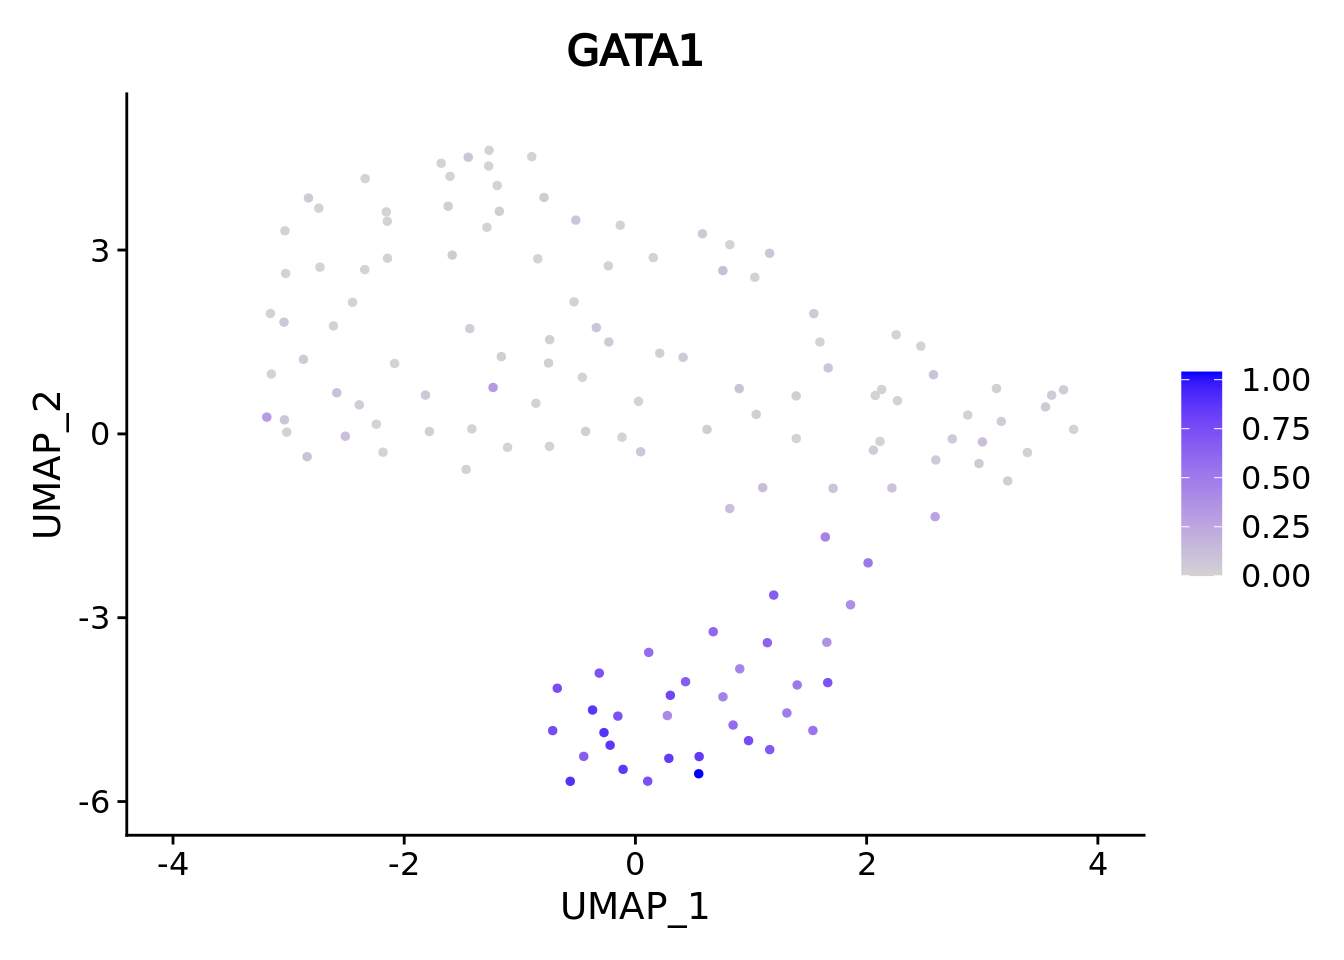
\includegraphics{21-MC_construction_discrete_files/figure-latex/unnamed-chunk-15-3.pdf}

\begin{Shaded}
\begin{Highlighting}[]
             
\NormalTok{mc\_QC.mc\_visualize\_continuous(ad, key}\OperatorTok{=}\StringTok{\textquotesingle{}X\_umap\textquotesingle{}}\NormalTok{, group\_by\_name}\OperatorTok{=}\StringTok{\textquotesingle{}membership\textquotesingle{}}\NormalTok{, }
\NormalTok{             colour\_sc\_name}\OperatorTok{=}\StringTok{\textquotesingle{}louvain\textquotesingle{}}\NormalTok{,  colour\_mc\_name}\OperatorTok{=}\StringTok{\textquotesingle{}Compactness\_PCA\textquotesingle{}}\NormalTok{, colour\_metacells}\OperatorTok{=}\VariableTok{True}\NormalTok{, }
\NormalTok{             legend\_sc}\OperatorTok{=}\VariableTok{None}\NormalTok{, legend\_mc}\OperatorTok{=}\StringTok{\textquotesingle{}auto\textquotesingle{}}\NormalTok{, metacell\_size}\OperatorTok{=}\DecValTok{30}\NormalTok{)   }
\end{Highlighting}
\end{Shaded}

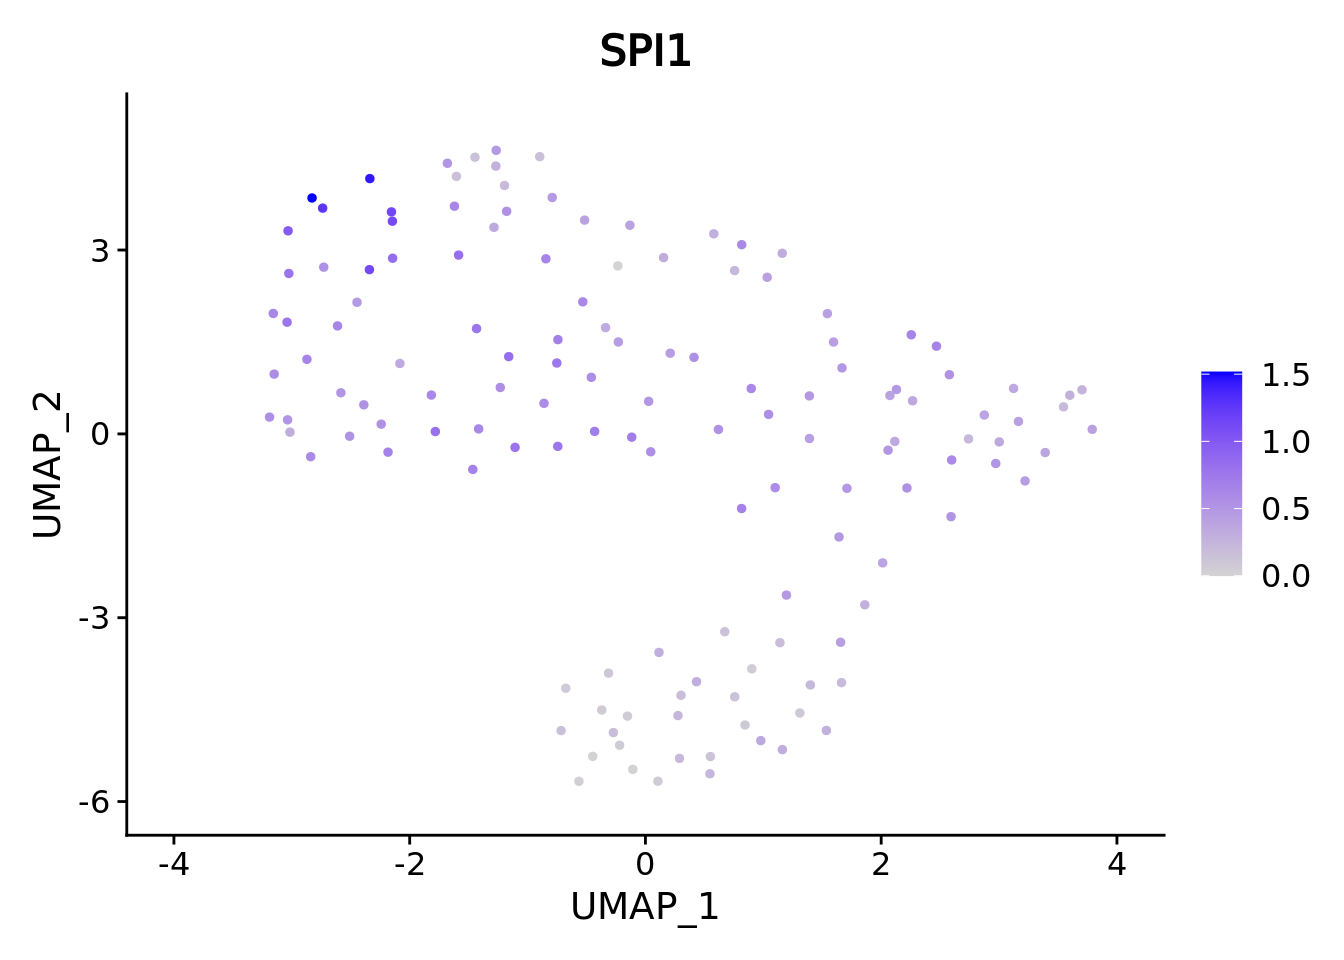
\includegraphics{21-MC_construction_discrete_files/figure-latex/unnamed-chunk-15-4.pdf}

\begin{Shaded}
\begin{Highlighting}[]
             
\NormalTok{mc\_QC.mc\_visualize\_continuous(ad, key}\OperatorTok{=}\StringTok{\textquotesingle{}X\_umap\textquotesingle{}}\NormalTok{, group\_by\_name}\OperatorTok{=}\StringTok{\textquotesingle{}membership\textquotesingle{}}\NormalTok{, }
\NormalTok{             colour\_sc\_name}\OperatorTok{=}\StringTok{\textquotesingle{}louvain\textquotesingle{}}\NormalTok{,  colour\_mc\_name}\OperatorTok{=}\StringTok{\textquotesingle{}Separation\_PCA\textquotesingle{}}\NormalTok{, colour\_metacells}\OperatorTok{=}\VariableTok{True}\NormalTok{, }
\NormalTok{             legend\_sc}\OperatorTok{=}\VariableTok{None}\NormalTok{, legend\_mc}\OperatorTok{=}\StringTok{\textquotesingle{}auto\textquotesingle{}}\NormalTok{, metacell\_size}\OperatorTok{=}\DecValTok{30}\NormalTok{)   }
\end{Highlighting}
\end{Shaded}

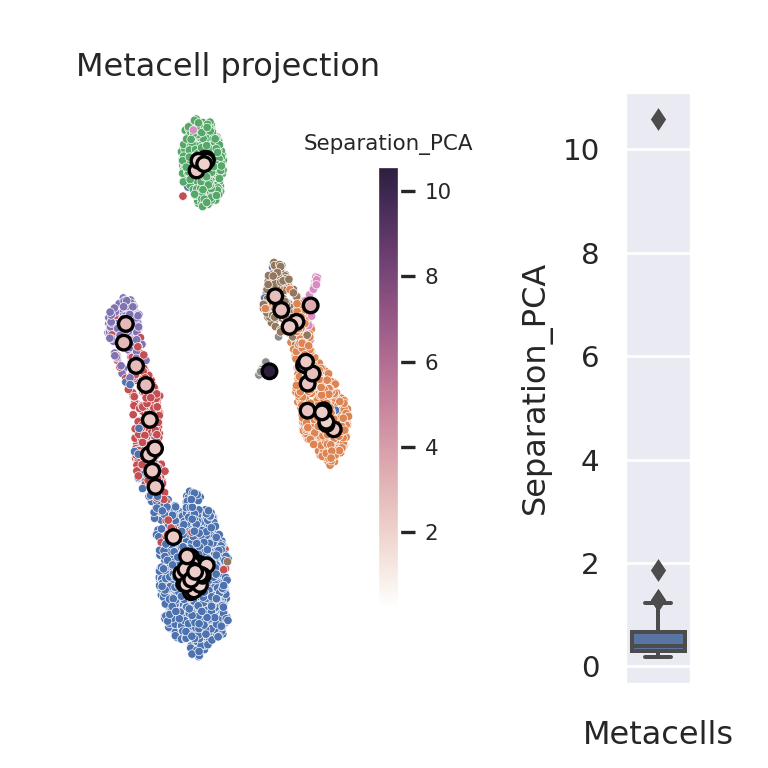
\includegraphics{21-MC_construction_discrete_files/figure-latex/unnamed-chunk-15-5.pdf}

\begin{Shaded}
\begin{Highlighting}[]
             
\CommentTok{\# mc\_QC.mc\_visualize\_continuous(ad, key=\textquotesingle{}X\_umap\textquotesingle{}, group\_by\_name=\textquotesingle{}membership\textquotesingle{},}
\CommentTok{\#              colour\_sc\_name=\textquotesingle{}louvain\textquotesingle{},  colour\_mc\_name=\textquotesingle{}INV\textquotesingle{}, colour\_metacells=True,}
\CommentTok{\#              legend\_sc=None, legend\_mc=\textquotesingle{}auto\textquotesingle{}, metacell\_size=30)}
\end{Highlighting}
\end{Shaded}

\hypertarget{save-output}{%
\paragraph*{Save output}\label{save-output}}
\addcontentsline{toc}{paragraph}{Save output}

\begin{Shaded}
\begin{Highlighting}[]
\NormalTok{mc\_ad.write\_h5ad(os.path.join(}\StringTok{\textquotesingle{}./data\textquotesingle{}}\NormalTok{, proj\_name, }\SpecialStringTok{f\textquotesingle{}metacell\_}\SpecialCharTok{\{}\NormalTok{MC\_tool}\SpecialCharTok{\}}\SpecialStringTok{.h5ad\textquotesingle{}}\NormalTok{))}
\end{Highlighting}
\end{Shaded}

\hypertarget{downstream-analysis-of-metacells-for-a-discrete-dataset}{%
\chapter{Downstream analysis of metacells (for a discrete dataset)}\label{downstream-analysis-of-metacells-for-a-discrete-dataset}}

Here we use the obtained metacell to run the downstream analysis on them instead of single-cell data. In this analysis, we treat metacell as single cell, neglecting information about their size (i.e., number of containing single cells). If you are interested in sample-weighted analysis, where metacell size is taken into account, see section \ref{weighted-analysis}.

\hypertarget{standard-analysis-r}{%
\section{Standard analysis (R)}\label{standard-analysis-r}}

Standard analysis includes dimensionality reduction, clustering, differential expression etc using Seurat {[}ref{]} framework.

Under construction\ldots{}

\hypertarget{dimensionality-reduction}{%
\subsection{Dimensionality reduction}\label{dimensionality-reduction}}

\hypertarget{clustering}{%
\subsection{Clustering}\label{clustering}}

\hypertarget{differential-expression-analysis}{%
\subsection{Differential expression analysis}\label{differential-expression-analysis}}

\hypertarget{standard-analysis-Py}{%
\section{Standard analysis (Python)}\label{standard-analysis-Py}}

Standard analysis includes dimensionality reduction, clustering, differential expression etc using \href{https://scanpy-tutorials.readthedocs.io/en/latest/\#}{Scanpy} framework.

Under construction\ldots{}

\hypertarget{dimensionality-reduction-1}{%
\subsection{Dimensionality reduction}\label{dimensionality-reduction-1}}

\hypertarget{clustering-1}{%
\subsection{Clustering}\label{clustering-1}}

\hypertarget{differential-expression-analysis-1}{%
\subsection{Differential expression analysis}\label{differential-expression-analysis-1}}

\hypertarget{advanced-analysis}{%
\section{Advanced analysis}\label{advanced-analysis}}

\hypertarget{grn}{%
\subsection{GRN}\label{grn}}

Gene correlation analysis suffers from large dropout rate of single-cell data and at the same time is very time and memory demanding. Metacells simultaneously adress both issues and thus are beneficial for gene co-expression and gene regulation analysis. Here we demonstrate usage of metacells for GRN analysis using SCENIC {[}ref{]}.

\hypertarget{weighted-analysis}{%
\section{Sample-weighted analysis}\label{weighted-analysis}}

One of the features of metacells are their size, which is a number of single cell it contains. Since metacells aggregate different number of cells, they also carry different amount of information. And thus, to better reproduce single-cell analysis, bigger metacells should have larger impact on the results than smaller metacells. For this, a sample-weighted analysis can be applied. Sample-weighted analysis is impleented in the SuperCell package.

\hypertarget{command-line-tool-for-mc-construction}{%
\chapter{Command line tool for MC construction}\label{command-line-tool-for-mc-construction}}

Here is a command line tool to construct metacells using either tool (MC2, SuperCell or SEACells) from a provided dataset.

\hypertarget{comparison-of-metacells-usage-for-a-discrete-and-continuous-data}{%
\chapter{Comparison of metacells usage for a discrete and continuous data}\label{comparison-of-metacells-usage-for-a-discrete-and-continuous-data}}

Under construction\ldots{}

\hypertarget{continuous-metacells-have-lower-purity}{%
\section{Continuous metacells have lower purity}\label{continuous-metacells-have-lower-purity}}

Under construction\ldots{}

\hypertarget{data-integration-with-metacells}{%
\chapter{Data integration with metacells}\label{data-integration-with-metacells}}

Under construction\ldots{}

  \bibliography{packages.bib}

\end{document}
